\documentclass[aspectratio=169]{beamer}
\usetheme{Madrid}

\usepackage{tikz}
\usepackage{url}

\usepackage{minted}
\usepackage{amsmath}

\title{Intro to \LaTeX}
\author{Andrew Huang}

\institute[University of Melbourne]

\titlegraphic{
	
\includegraphics[height=0.1\linewidth]{./Images/mueec_logo.png}
	\hspace{2.5cm}
	
\includegraphics[height=0.1\linewidth]{./Images/arrp_logo.png}
}

\AtBeginSection[]
{
	\begin{frame}<beamer>{Outline}
		\tableofcontents[currentsection,currentsubsection]
	\end{frame}
}

\newcommand\blfootnote[1]{%
	\begingroup
	\renewcommand\thefootnote{}\footnote{#1}%
	\addtocounter{footnote}{-1}%
	\endgroup
}

\begin{document}
\begin{frame}
    \maketitle
\end{frame}

\begin{frame}{Outline}
	\tableofcontents
\end{frame}

\section{Why \LaTeX?}
%!TeX root = main.tex

\begin{frame}{\insertsection}
	\begin{figure}
		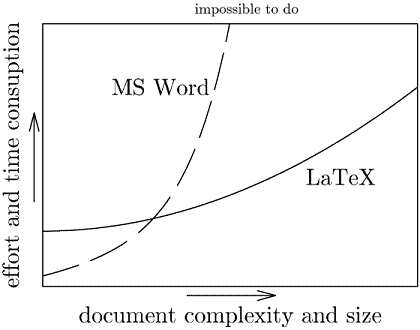
\includegraphics[scale=0.5]{./Images/latex-difficulty-2.png}
	\end{figure}
\end{frame}

\begin{frame}{\insertsection}{Work flow improvements}
	\begin{figure}
		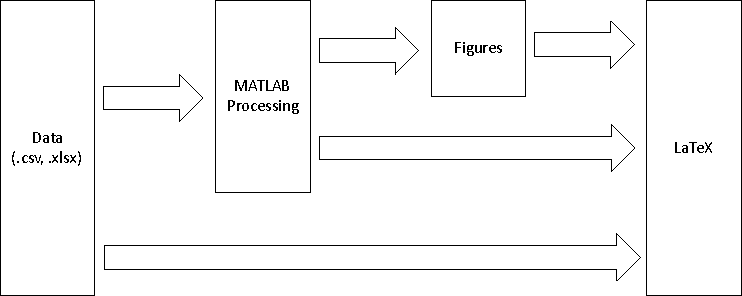
\includegraphics[width=0.7\linewidth]{./Images/workflow.pdf}
	\end{figure}
\end{frame}

\begin{frame}{\insertsection}{Pretty Pictures}
	\begin{figure}
		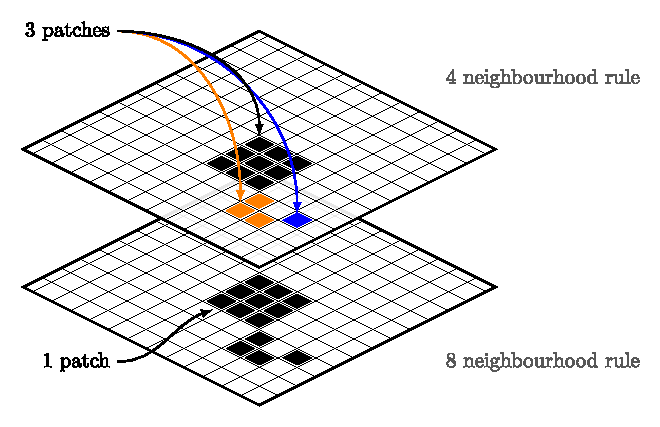
\includegraphics[width=0.35\linewidth]{./Images/Neighbourhood_definition2.pdf}
		\hspace{5em}
		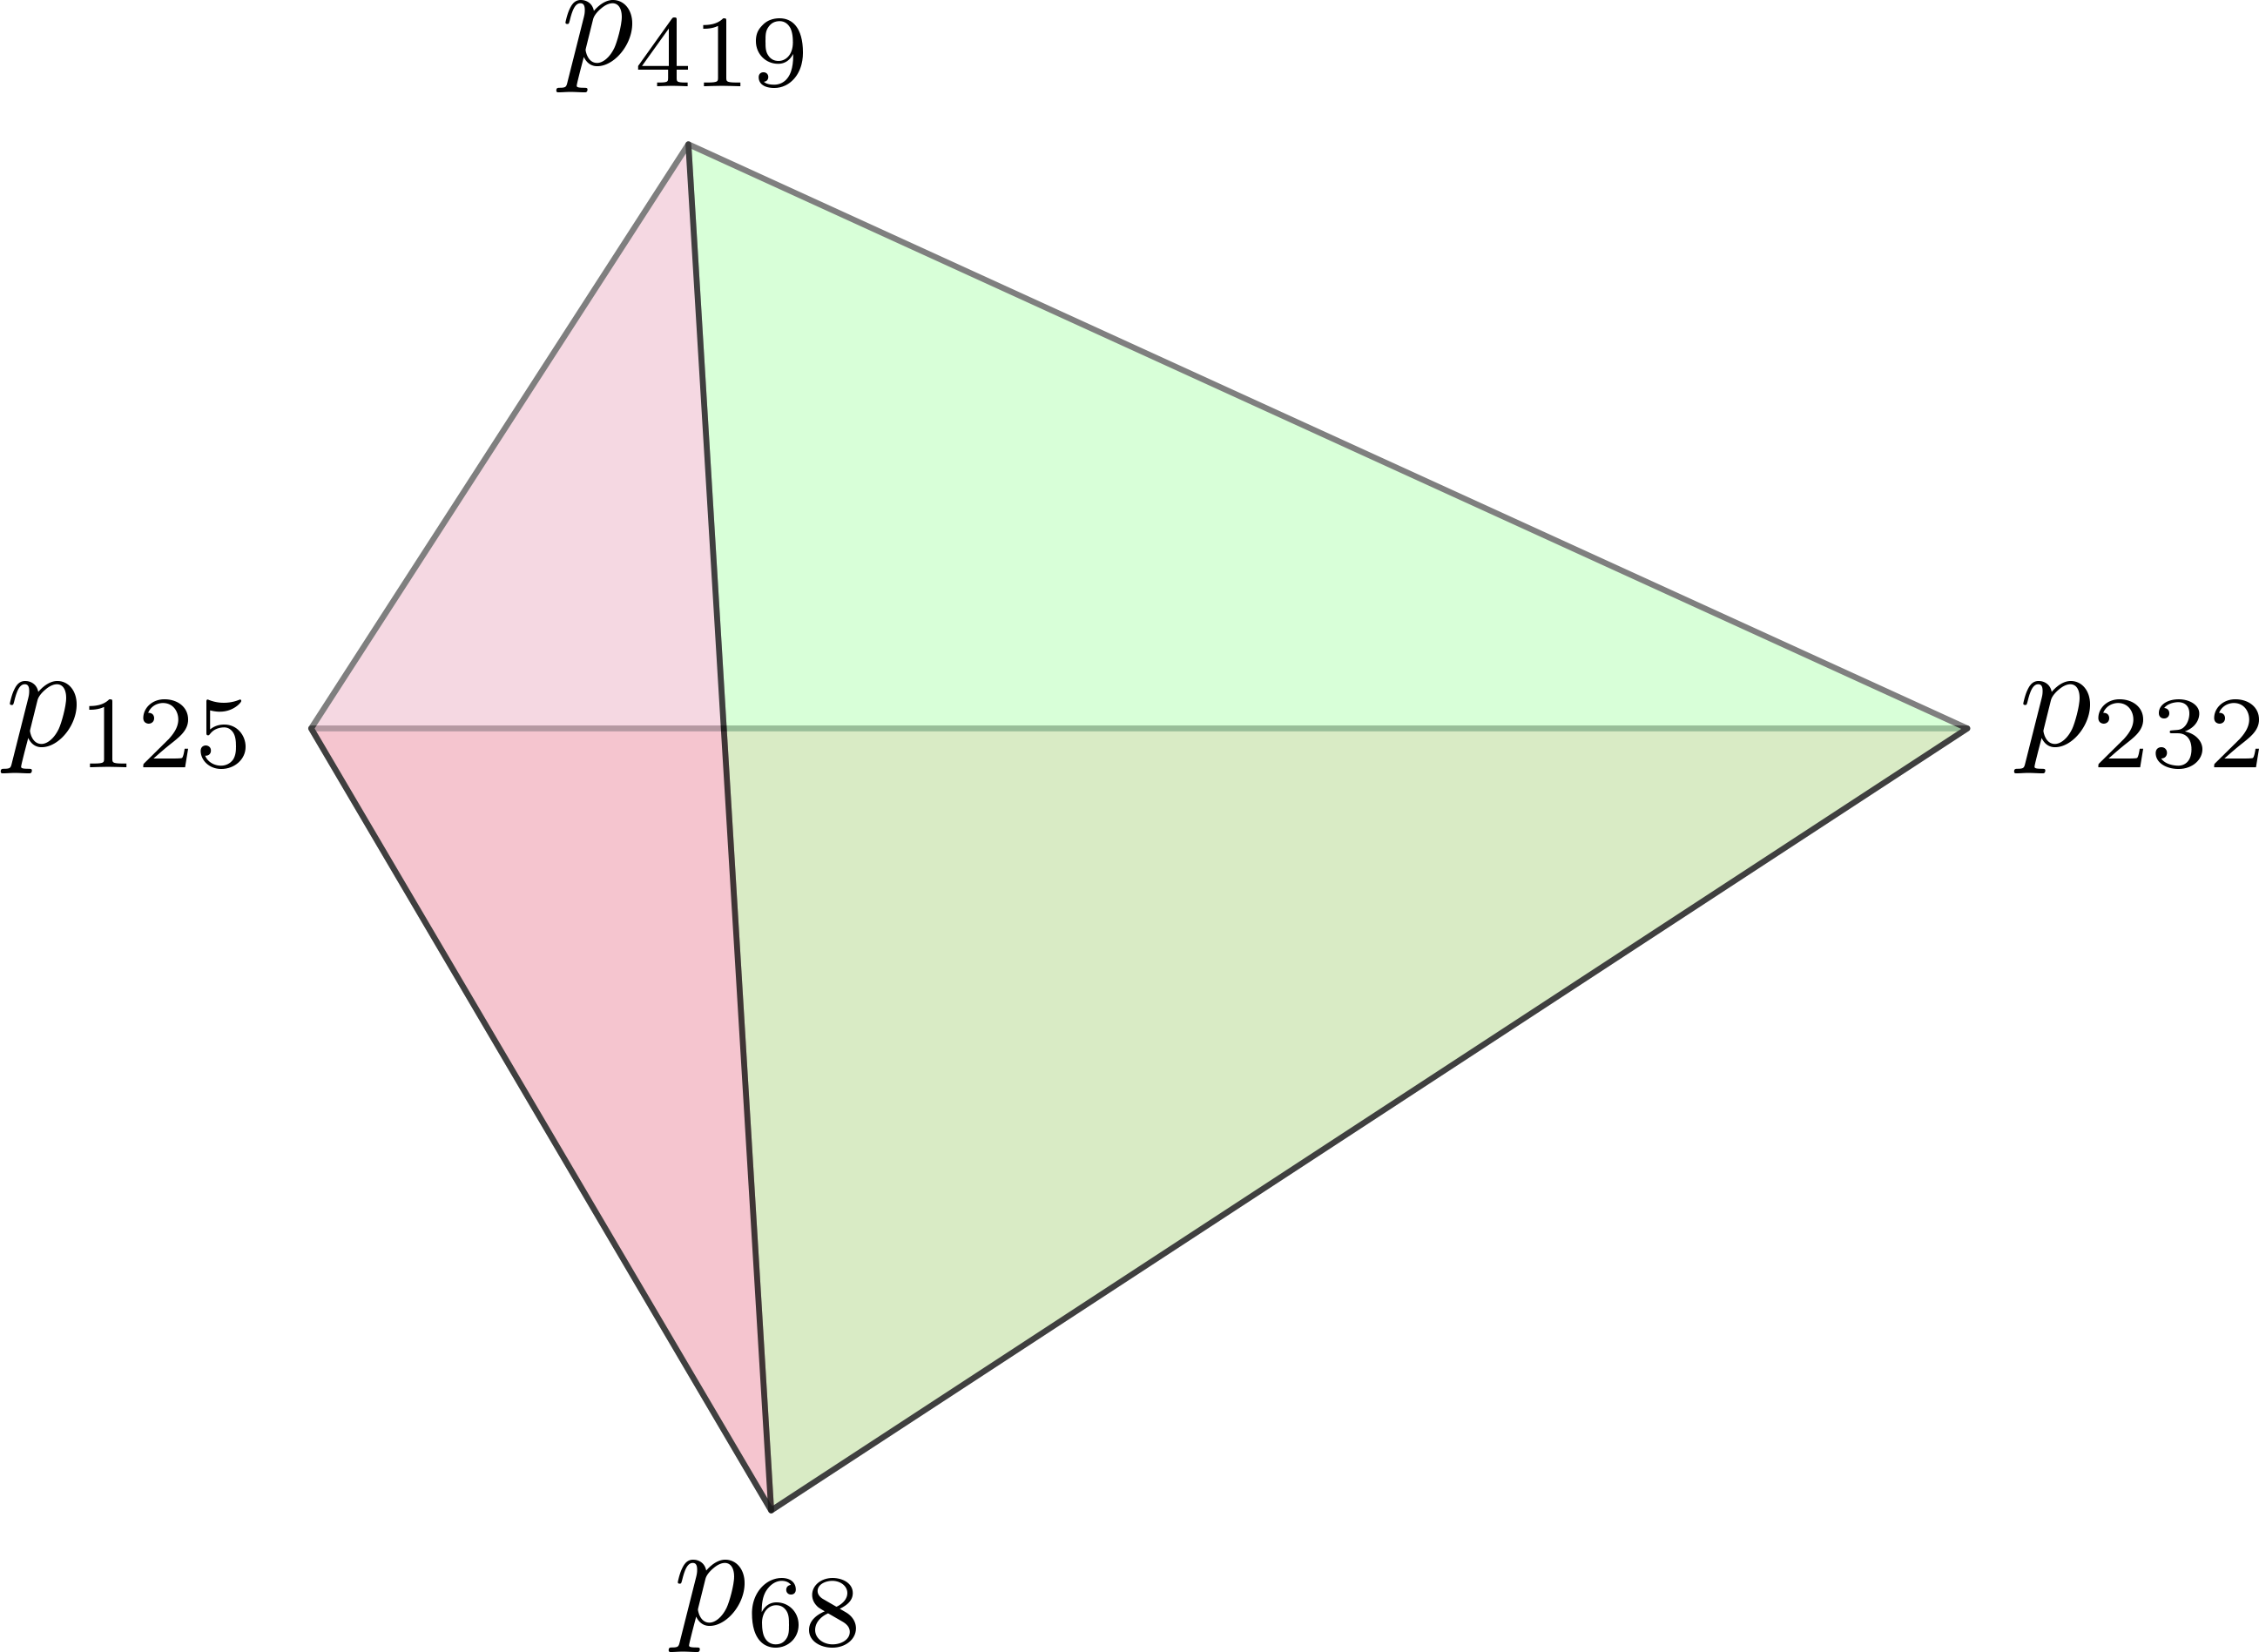
\includegraphics[width=0.35\linewidth]{./Images/nicePic.png}
	\end{figure}
	\blfootnote{PGF -- \url{https://ctan.org/pkg/pgf?lang=en}}
\end{frame}

\begin{frame}{\insertsection}{Circuitry}
	\begin{figure}
		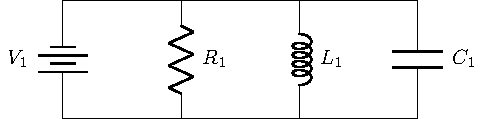
\includegraphics[width=0.7\linewidth]{./LaTex_Tikz/circuitikz.pdf}
	\end{figure}
	\blfootnote{circuitikz -- \url{https://ctan.org/pkg/circuitikz?lang=en}}
\end{frame}

\begin{frame}{\insertsection}{Presentation}
	\begin{figure}
		
\includegraphics[width=0.4\linewidth]{./Images/beamer.png}
	\end{figure}
	\blfootnote{Beamer Class -- \url{https://ctan.org/pkg/beamer?lang=en}}
\end{frame}

\begin{frame}{\insertsection}{Exams}
	\begin{figure}
		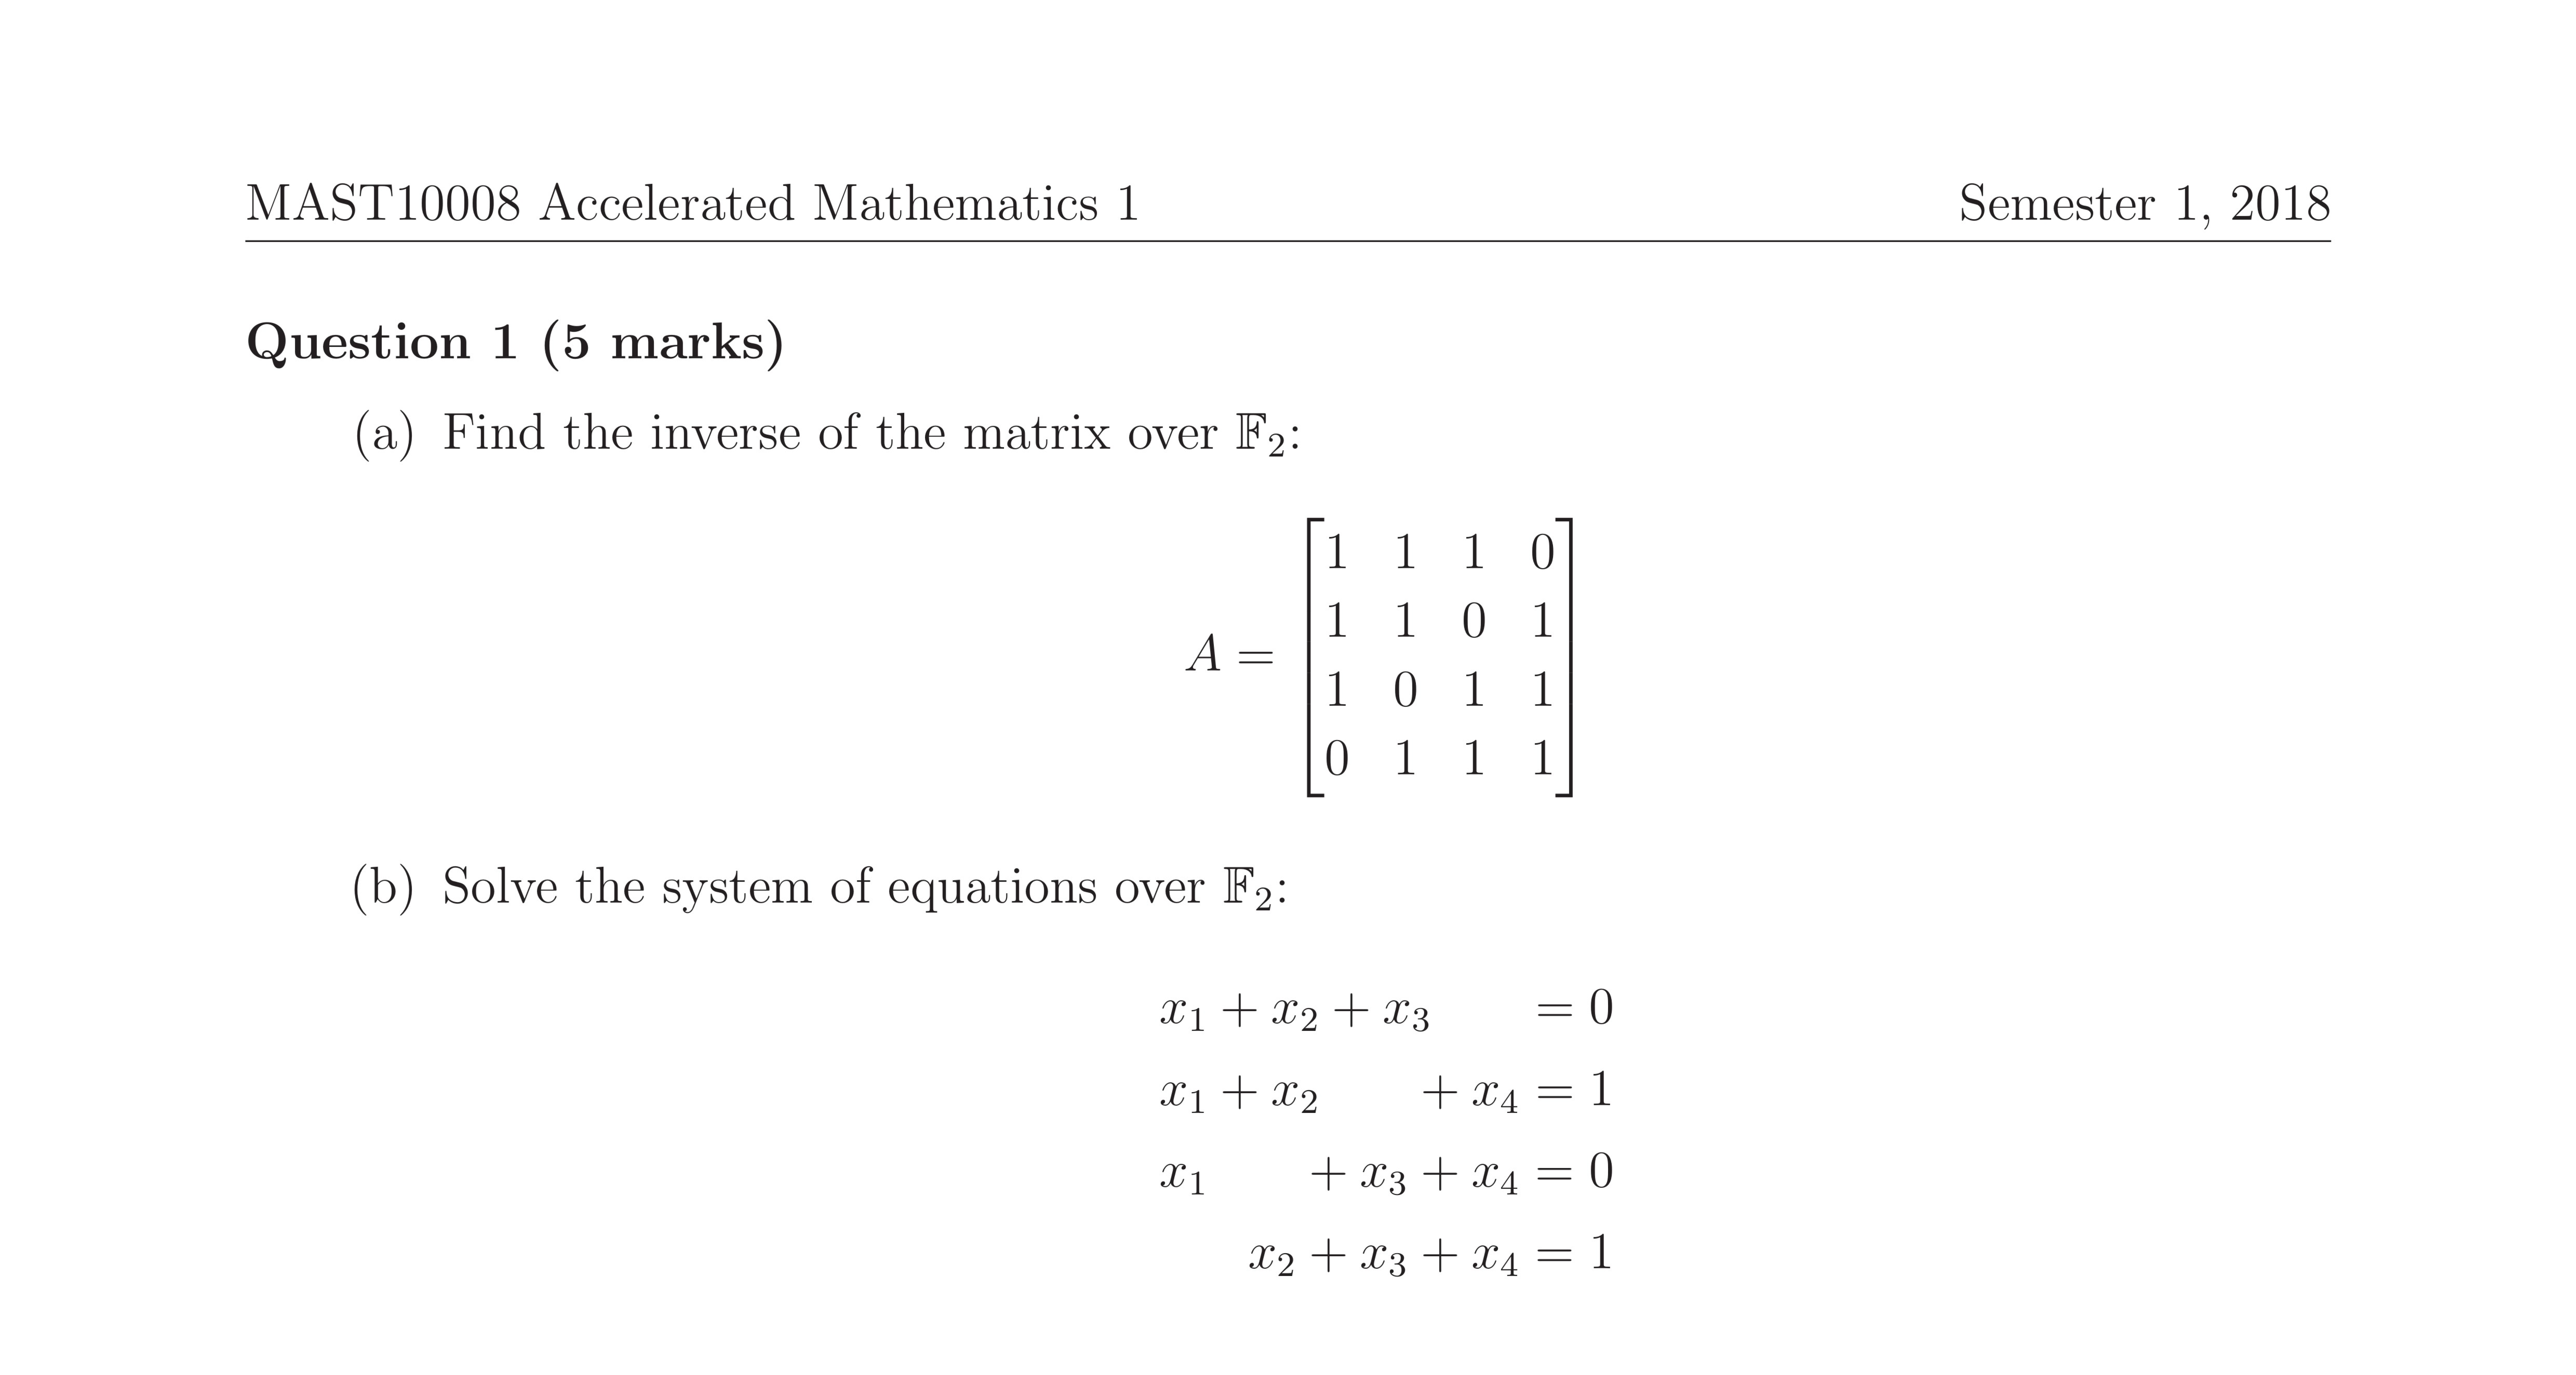
\includegraphics[width=0.4\linewidth]{./Images/AM1-2.png}
		\hspace{5em}
		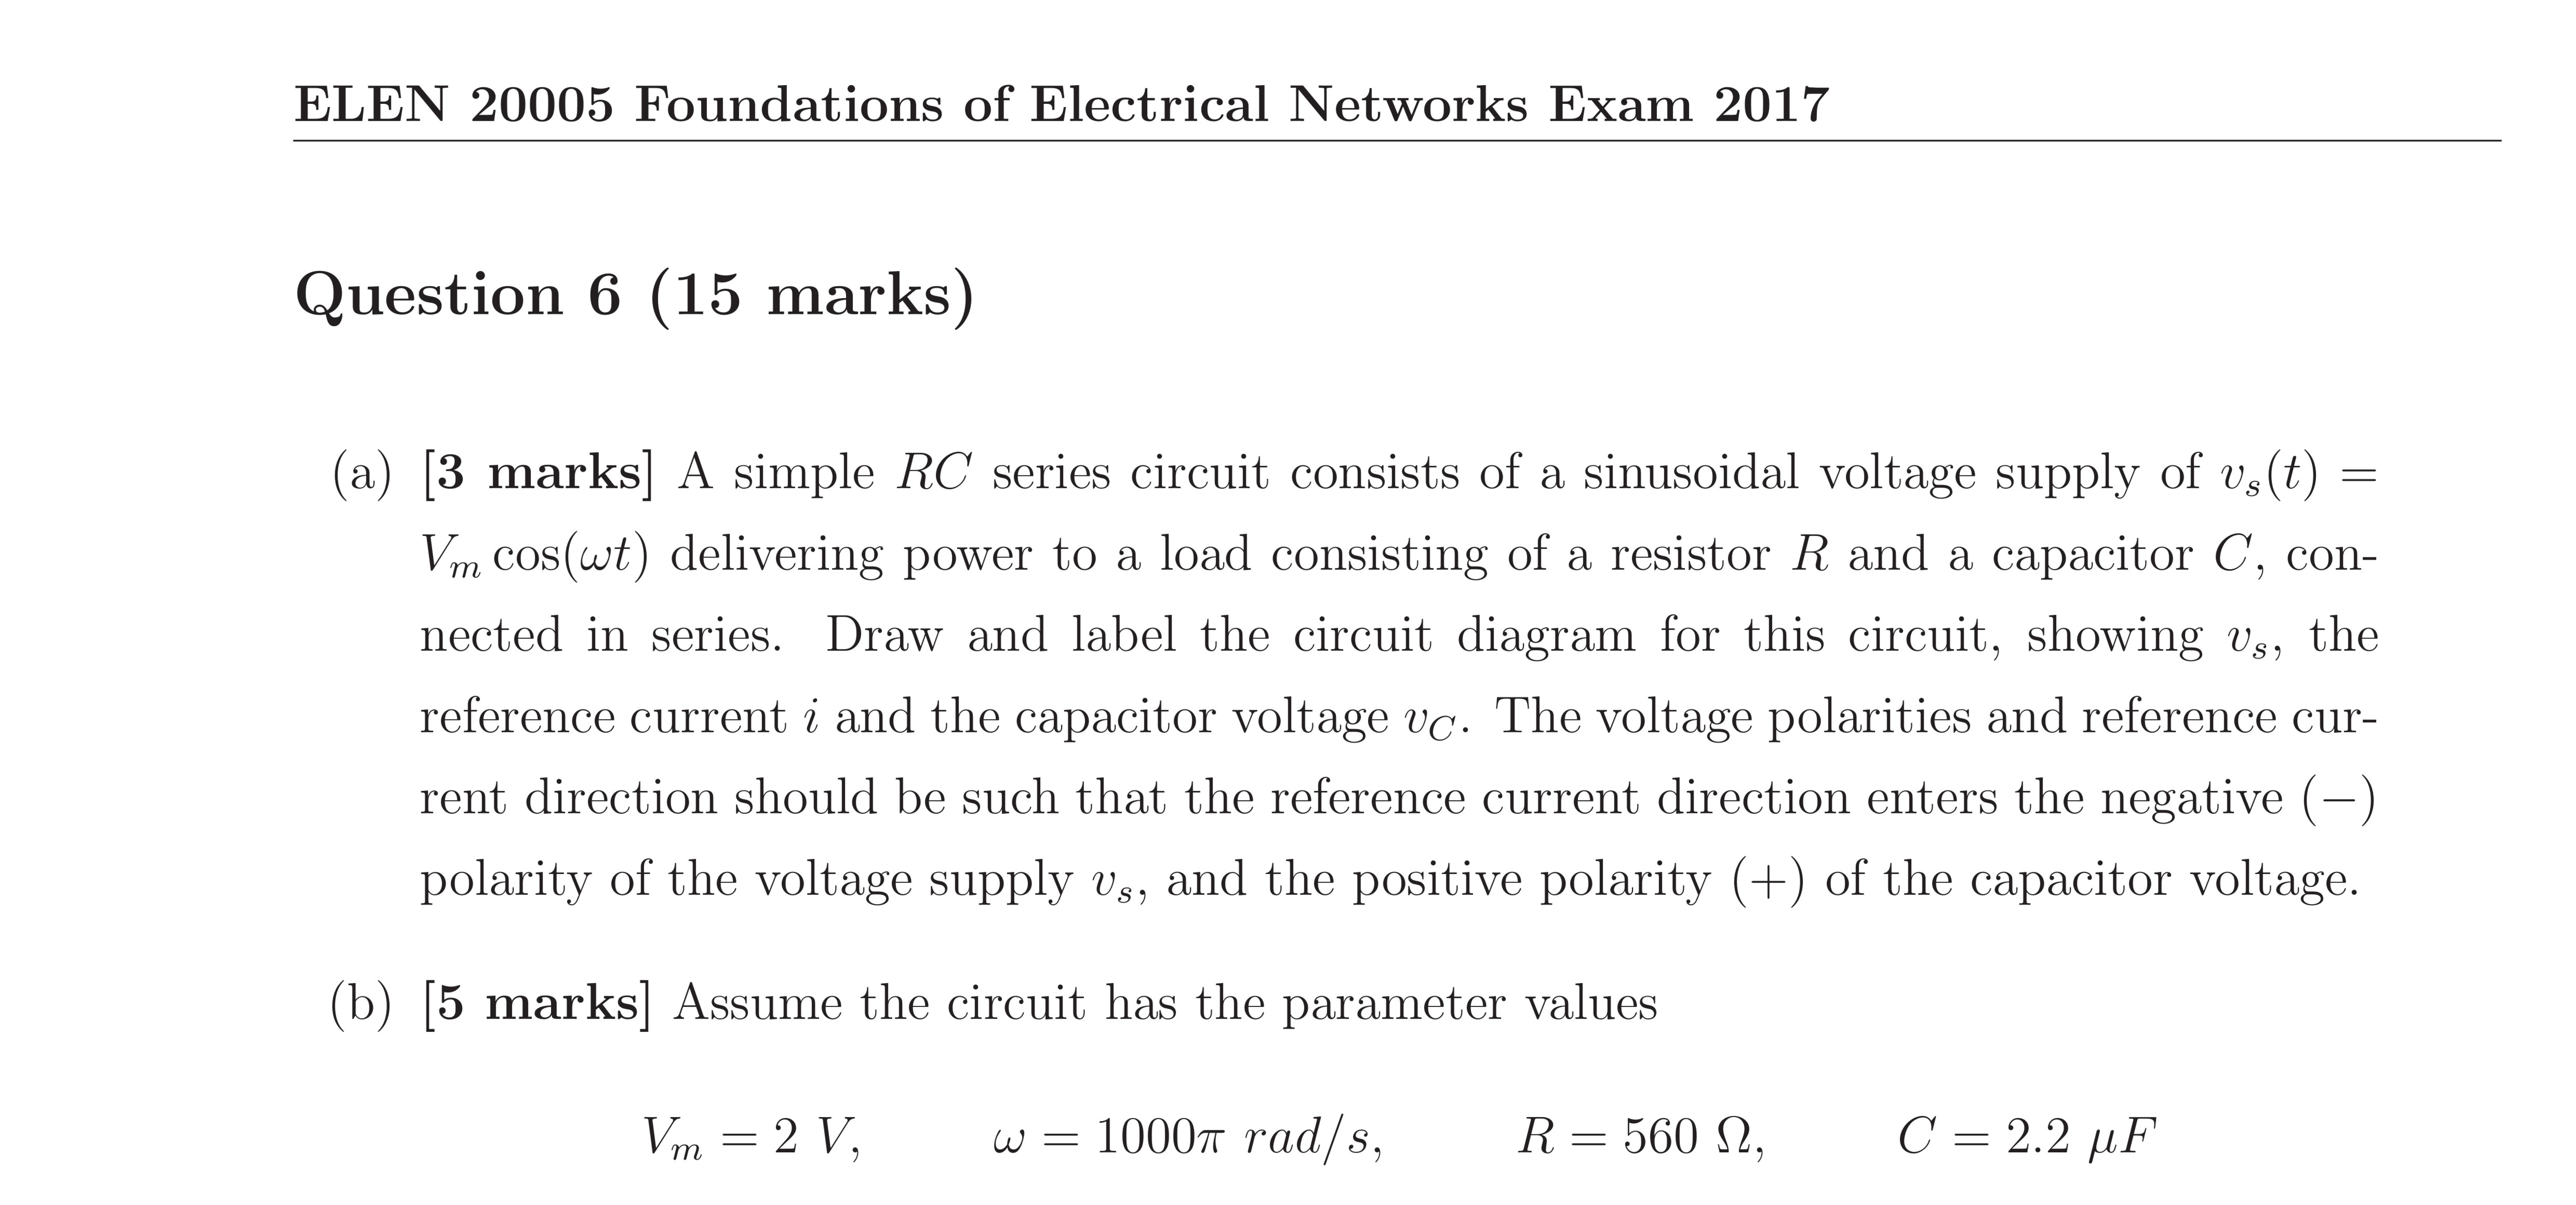
\includegraphics[width=0.4\linewidth]{./Images/elen.png}
	\end{figure}
	\blfootnote{Exam Class -- \url{https://ctan.org/pkg/exam?lang=en}}
\end{frame}

\begin{frame}{\insertsection}{Code Highlighting}
	\tiny{\inputminted[numbers=none, frame=single]{matlab}{./Example_Codes/A_over_Astar_isentropic.m}}
	\blfootnote{Exam Class -- \url{https://ctan.org/pkg/exam?lang=en}}
\end{frame}

\begin{frame}{\insertsection}{}
	\centering
	\Huge{Most Importantly}
\end{frame}

\begin{frame}{\insertsection}{Academically Professional}
	\begin{figure}
		
\includegraphics[height=0.7\textheight]{./Images/file_extensions_2x.png}
		\hspace{5em}
		
\includegraphics[height=0.7\textheight]{./Images/latex.png}
	\end{figure}
\end{frame}

\section{How to get started}
%!TeX root = main.tex

\begin{frame}{\insertsection}{}
	\begin{itemize}
		\item Working Online
		\begin{itemize}
			\item Overleaf
			\begin{itemize}
				\item University of Melbourne, has a campus subscription to Overleaf
			\end{itemize}
				\item \LaTeX\ Base
				\item Papeeria
		\end{itemize}
		\item Working Offline
		\begin{itemize}
			\item \LaTeX\ Distributions
			\begin{itemize}
				\item MiKTex
				\item Tex Live
			\end{itemize}
			\item Third-part Editors
			\begin{itemize}
				\item TeX Studio
				\item TeX Maker
				\item Visual Studio Code
				\item Notepad
			\end{itemize}
		\end{itemize}
	\end{itemize}
\end{frame}

\begin{frame}{\insertsection}{Your First Document}
	\begin{block}{Hello World.tex}
		\inputminted[numbers=none]{latex}{./Example_Codes/FirstDoc.tex}
	\end{block}
\end{frame}

\begin{frame}{\insertsection}{Customization}
	\begin{block}{Custom Margins and Paper size}
		\inputminted[numbers=none]{latex}{./Example_Codes/SecDoc.tex}
	\end{block}
\end{frame}

\begin{frame}{\insertsection}{Text Emphasis}
	\begin{block}{Bold}
		{\mintinline{latex}{\textbf{text}}}
	\end{block}
	\begin{block}{Italics}
		{\mintinline{latex}{\textit{text}}}
	\end{block}
	\begin{block}{Underlined}
		{\mintinline{latex}{\underline{text}}}
	\end{block}
\end{frame}

\begin{frame}{\insertsection}{Images}
	\begin{block}{Images Style 1}
	\inputminted[numbers=none]{latex}{./Example_Codes/images1.tex}
	\end{block}
\end{frame}

\begin{frame}{\insertsection}{Images}
	\begin{block}{Images Style 2}
		\inputminted[numbers=none]{latex}{./Example_Codes/images2.tex}
	\end{block}
\end{frame}

\begin{frame}{\insertsection}{Math typing and the \mintinline{latex}{amsmath} package}
	\mintinline{latex}{\usepackage{amsmath}}
	\begin{block}{Numbered environments}
		\mintinline{latex}{eqaution}, \mintinline{latex}{gather}, \mintinline{latex}{align}
	\end{block}
	\begin{block}{Unnumbered environments}
		\mintinline{latex}{eqaution*}, \mintinline{latex}{gather*}, \mintinline{latex}{align*}
	\end{block}
	\begin{block}{Inline}
		\mintinline{latex}{$y = mx + c$}
	\end{block}
\end{frame}

\begin{frame}{\insertsection}{Sectioning}
	\mintinline{latex}{\tableofcontents}
	\begin{block}{Numbered}
		\mintinline{latex}{\section{Text}}, \mintinline{latex}{\subsection{Text}} ...
	\end{block}
	\begin{block}{Unnumbered}
	\mintinline{latex}{\section*{Text}}, \mintinline{latex}{\subsection*{Text}} ...
	\end{block}
\end{frame}

\begin{frame}{\insertsection}{Tables}
		\begin{block}{Example Table}
		\inputminted[numbers=none]{latex}{./Example_Codes/table.tex}
	\end{block}
\end{frame}

\begin{frame}{\insertsection}{Tables}
	\begin{figure}
		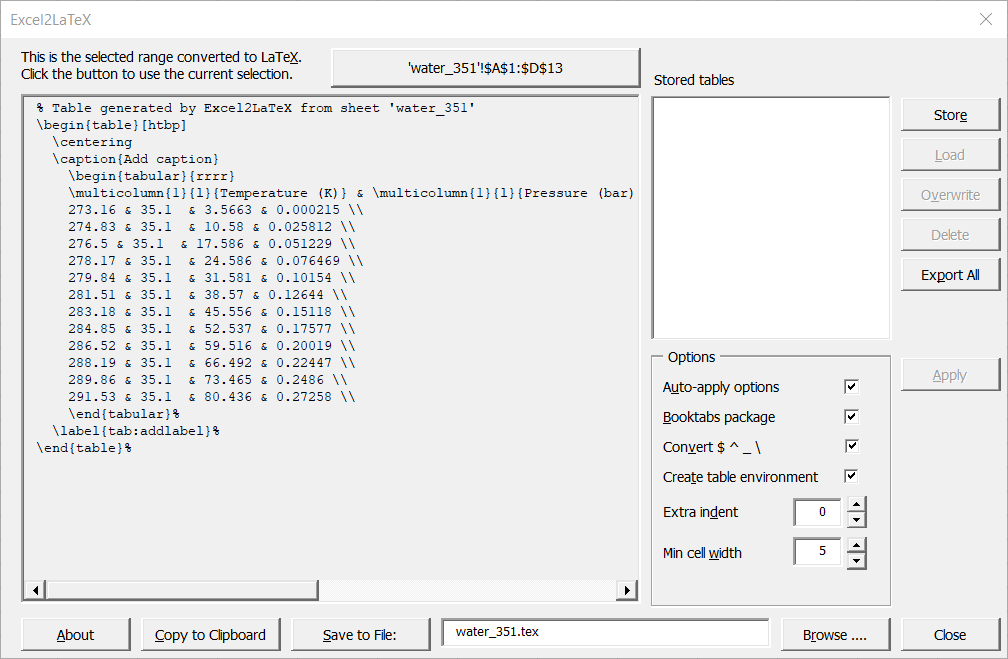
\includegraphics[width=0.4\textwidth]{./Images/excel2latex.png}
	\end{figure}
	Use Excel2LaTeX instead, it provides automatic generation of \LaTeX\ code from excel sheets.
	\blfootnote{Excel2LaTeX -- \url{https://ctan.org/pkg/excel2latex?lang=en}}
\end{frame}

\begin{frame}{Other Nice Packages}
	\begin{itemize}
		\item \mintinline{latex}{amssymb}\\
		More mathematical symbols from AMS
		\item \mintinline{latex}{pdfpages}\\
		Ability to include and splice external PDFs into your \LaTeX\ document
		\item \mintinline{latex}{siunitx}\\
		SI unit formatting and decimal alignment in tables
		\item \mintinline{latex}{csvsimple}\\
		Read .csv files to automatically create tables
		\item \mintinline{latex}{booktabs}\\
		Nicer looking table dividers
		\item \mintinline{latex}{fancyhdr}\\	
		Headers for documents	
	\end{itemize}
\end{frame}

\begin{frame}{Complimentary Programs}
	\begin{itemize}
		\item IguanaTeX\\
		\LaTeX\ in Power Points
		\item Inkscape\\
		Vector image editor
		\item Microsoft Visio\\
		Visual editor for flowcharts and diagrams\\
		My addon for \LaTeX\ in Visio (\url{https://github.com/huanga2/VSTO_LaTeX})
	\end{itemize}
\end{frame}

\begin{frame}{Further sources}
	\begin{itemize}
		\item Google
		\item TeX StackExchange
		\item Comprehensive TeX Archive Network -- \url{https://ctan.org/}
		\item Overleaf
		\item Math symbols -- \url{https://oeis.org/wiki/List_of_LaTeX_mathematical_symbols}
	\end{itemize}
\end{frame}

\section{Exercise}
%!TeX root = main.tex

\begin{frame}{\insertsection}{}
	\centering
	\Huge{Use any past assignments or tutorial worksheets, or use the next slide}
\end{frame}

\begin{frame}{\insertsection}{}
	\centering
	\begin{minipage}{0.8\textwidth}
		\textbf{Question 2 (4 marks)}\\
		Use the principle of mathematical induction to prove that, for any $n \in \mathbb{N}$, the $n$-th derivative of $f(x) = x^2e^x$ is $\left(n(n-1) + 2nx + x^2\right) e^x$. \vspace{1em}\\
		\textbf{Question 3 (10 marks)}\\
		Let $L_1$ be the line in $\mathbb{R}^3$ with the vector equation
		\begin{equation*}
			(x, y, z) = (k, -1, 1) + t(1, 0, -1), \quad t \in \mathbb{R}
		\end{equation*}
		where $k$ is a real constant, and let $L_2$ be the line $\mathbb{R}^3$  with Cartesian equations
		\begin{equation*}
			\dfrac{x+1}{2} = \dfrac{y + 5}{4} = z - 2
		\end{equation*}
	\end{minipage}
\end{frame}

\end{document}
